\documentclass{article}
\usepackage{iclr2027_conference,times}


\usepackage[utf8]{inputenc}
\usepackage[T1]{fontenc}
\usepackage{nicefrac}
\usepackage{microtype}
\usepackage{amsmath,amssymb,amsthm,mathrsfs}
\usepackage{algorithm}
\usepackage{algpseudocode}
\usepackage{graphicx}
\usepackage{pgfplots}
\usepackage{pgfplotstable}
\pgfplotsset{compat=1.18}
\usepackage{tikz}
\usetikzlibrary{arrows.meta,calc,positioning,patterns,shapes.arrows,fit,backgrounds}
\usepackage{array}
\usepackage{booktabs}
\usepackage{colortbl}
\usepackage{longtable}
\usepackage[most]{tcolorbox}
\usepackage{float}
\usepackage{placeins}
\usepackage{chemfig}
\usepackage{xcolor}
\usepackage{url}
\usepackage[hidelinks]{hyperref}


\iclrfinalcopy
\begin{document}
\newbox\exportbox
\setbox\exportbox=\hbox{\resizebox{\textwidth}{!}{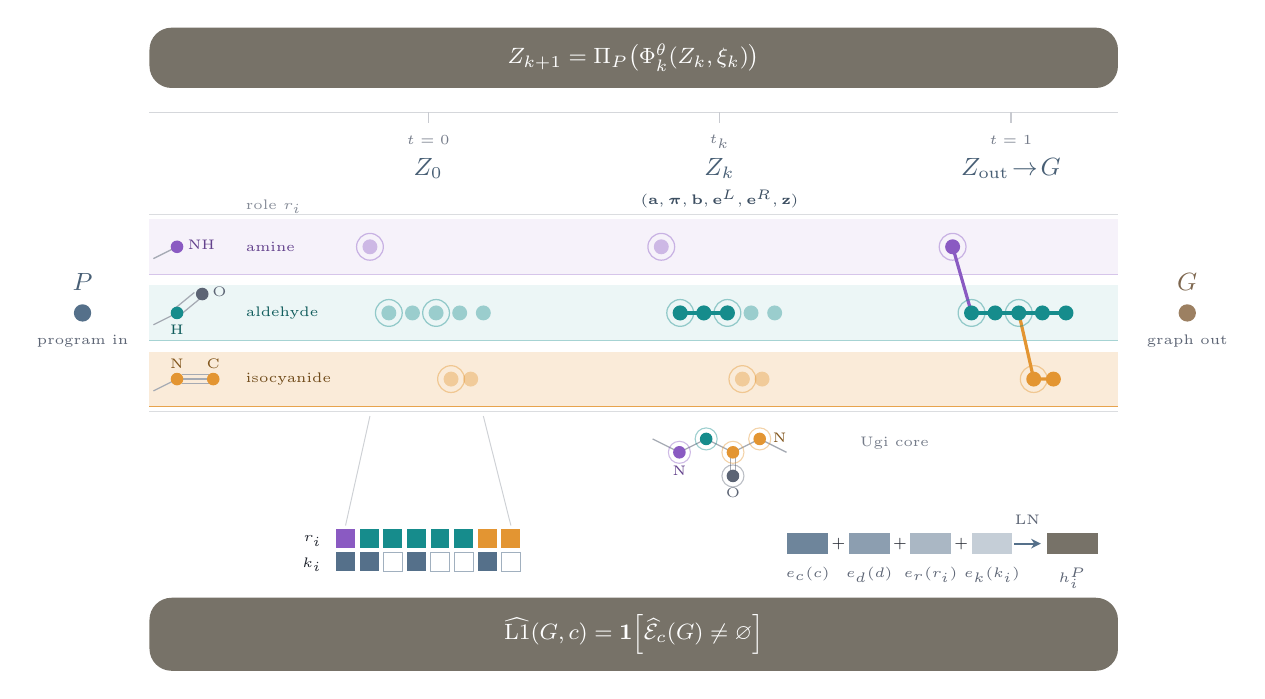
\begin{tikzpicture}[
  font=\scriptsize,
  plate/.style={rounded corners=8pt, fill=navybar, fill opacity=0.79, text opacity=1, text=white, inner xsep=10pt, inner ysep=6pt,
    minimum width=12.30cm, align=center, font=\footnotesize},
  statelab/.style={text=peri!85!black, font=\small},
  lead/.style={-{Stealth[length=3pt,width=3pt]}, draw=peri!75, line width=0.6pt},
]
\definecolor{roleamine}{HTML}{8A5AC2}
\definecolor{roleald}{HTML}{168C8C}
\definecolor{roleiso}{HTML}{E39532}
\definecolor{ground}{HTML}{F4F1E9}
\definecolor{groundcore}{HTML}{D9C9A6}
\colorlet{navybar}{groundcore!38!black}
\definecolor{peri}{HTML}{55708A}
\definecolor{cyanacc}{HTML}{9C8062}
\definecolor{ink}{HTML}{22262F}
\definecolor{inkmuted}{HTML}{5C6474}

\def\sxa{4.54}     \def\cx{8.24}
\def\sxc{11.94}
\def\bandl{1.00}
\def\bandr{13.30}
\def\platecx{7.15}
\def\labx{2.10}    \def\inx{0.15}     \def\outx{14.18}   \def\ya{0.05}      \def\yaxis{2.60}   \def\ypanel{-3.15} \def\bandh{0.35}   

\foreach \sy/\col/\bandop/\ruleop/\labmix/\lb in {8.4/roleamine/0.079/0.35/72/{amine}/{$\mathrm{N}\text{--}\mathrm{H}$},
       0.0/roleald/0.084/0.38/65/{aldehyde}/{$\mathrm{CH}{=}\mathrm{O}$},
      -8.4/roleiso/0.186/0.84/49/{isocyanide}/{$\mathrm{N}{\equiv}\mathrm{C}$}} {
  \pgfmathsetmacro\yc{\ya+\sy/10}
  \pgfmathsetmacro\ytop{\yc+\bandh}
  \pgfmathsetmacro\ybot{\yc-\bandh}
  \fill[\col, opacity=\bandop] (\bandl,\ybot) rectangle (\bandr,\ytop);
  \draw[\col, opacity=\ruleop, line width=0.4pt] (\bandl,\ybot) -- (\bandr,\ybot);
  \node[font=\tiny, text=\col!\labmix!black, anchor=west] at (\labx,\yc) {\lb};
}
\pgfmathsetmacro\blocktop{\ya+0.84+\bandh+0.06}
\pgfmathsetmacro\blockbot{\ya-0.84-\bandh-0.06}
\pgfmathsetmacro\rolehdr{\blocktop+0.10}
\draw[draw=inkmuted!22, line width=0.35pt] (\bandl,\blocktop) -- (\bandr,\blocktop);
\draw[draw=inkmuted!22, line width=0.35pt] (\bandl,\blockbot) -- (\bandr,\blockbot);
\node[font=\tiny, text=inkmuted!75, anchor=west] at (\labx,\rolehdr) {role $r_i$};

\tikzset{frag/.style={line width=0.45pt, draw=inkmuted!55}, lbl/.style={font=\tiny, inner sep=0.6pt}}
\begin{scope}[shift={(1.05,\ya+0.84)}]
  \draw[frag] (0mm,-1.5mm) -- (3.0mm,0mm);
  \fill[roleamine] (3.0mm,0mm) circle (0.8mm);
  \node[lbl, text=roleamine!72!black, anchor=west] at (4.1mm,0.2mm) {NH};
\end{scope}
\begin{scope}[shift={(1.05,\ya)}]
  \draw[frag] (0mm,-1.5mm) -- (3.0mm,0mm);
  \draw[frag] (2.65mm,0.5mm) -- (5.2mm,2.6mm);
  \draw[frag] (3.35mm,-0.3mm) -- (5.9mm,1.8mm);
  \fill[roleald] (3.0mm,0mm) circle (0.8mm);
  \fill[inkmuted] (6.2mm,2.4mm) circle (0.8mm);
  \node[lbl, text=inkmuted, anchor=west] at (7.2mm,2.7mm) {O};
  \node[lbl, text=roleald!65!black, anchor=north] at (3.0mm,-1.3mm) {H};
\end{scope}
\begin{scope}[shift={(1.05,\ya-0.84)}]
  \draw[frag] (0mm,-1.5mm) -- (3.0mm,0mm);
  \foreach \dy in {-0.55,0,0.55} \draw[frag] (3.6mm,\dy mm) -- (7.0mm,\dy mm);
  \fill[roleiso] (3.0mm,0mm) circle (0.8mm);
  \fill[roleiso] (7.6mm,0mm) circle (0.8mm);
  \node[lbl, text=roleiso!57!black, anchor=south] at (3.0mm,1.0mm) {N};
  \node[lbl, text=roleiso!57!black, anchor=south] at (7.6mm,1.0mm) {C};
\end{scope}


\fill[peri] (\inx,\ya) circle (1.1mm);
\node[font=\small, text=peri!85!black, anchor=south] at (\inx,\ya+0.16) {$P$};
\node[font=\tiny, text=inkmuted, anchor=north] at (\inx,\ya-0.16) {program in};
\fill[cyanacc] (\outx,\ya) circle (1.1mm);
\node[font=\small, text=cyanacc!80!black, anchor=south] at (\outx,\ya+0.16) {$G$};
\node[font=\tiny, text=inkmuted, anchor=north] at (\outx,\ya-0.16) {graph out};

\newcommand{\forgesites}[1]{\foreach \px/\py/\col/\core in {-7.4/8.4/roleamine/1,
      -5.0/0.0/roleald/1, -2.0/0.0/roleald/0, 1.0/0.0/roleald/1,
       4.0/0.0/roleald/0,  7.0/0.0/roleald/0,
       2.9/-8.4/roleiso/1,  5.4/-8.4/roleiso/0} {
    \ifnum\core=1 \draw[\col, line width=0.45pt, opacity=0.42] (\px mm,\py mm) circle (1.7mm); \fi
    \ifnum#1=1 \fill[\col] (\px mm,\py mm) circle (0.95mm);
    \else \fill[\col, opacity=0.38] (\px mm,\py mm) circle (0.95mm); \fi
  }}

\begin{scope}[shift={(\sxa,\ya)}] \forgesites{0} \end{scope}

\begin{scope}[shift={(\cx,\ya)}]
  \draw[roleald, line width=1.15pt] (-5mm,0mm) -- (-2mm,0mm) -- (1mm,0mm);
  \forgesites{0}
  \foreach \px in {-5.0, -2.0, 1.0} \fill[roleald] (\px mm,0mm) circle (0.95mm);
\end{scope}

\begin{scope}[shift={(\sxc,\ya)}]
  \draw[roleald, line width=1.15pt] (-5mm,0mm) -- (7mm,0mm);
  \draw[roleiso, line width=1.15pt] (1mm,0mm) -- (2.9mm,-8.4mm) -- (5.4mm,-8.4mm);
  \draw[roleamine, line width=1.15pt] (-5mm,0mm) -- (-7.4mm,8.4mm);
  \forgesites{1}
\end{scope}

\draw[draw=inkmuted!26, line width=0.4pt] (\bandl,\yaxis) -- (\bandr,\yaxis);
\foreach \tx/\tl/\sl in {\sxa/{$t=0$}/{$Z_0$}, \cx/{$t_k$}/{$Z_k$}, \sxc/{$t=1$}/{$Z_{\rm out}\!\to\!G$}} {
  \draw[draw=inkmuted!34, line width=0.5pt] (\tx,\yaxis) -- (\tx,\yaxis-0.14);
  \node[font=\tiny, text=inkmuted!85, anchor=north] at (\tx,\yaxis-0.17) {\tl};
  \node[statelab, anchor=north] at (\tx,\yaxis-0.47) {\sl};
}
\node[font=\tiny, text=peri!70!black, anchor=north] at (\cx,\yaxis-0.86)
  {$(\mathbf{a},\boldsymbol{\pi},\mathbf{b},\mathbf{e}^{L},\mathbf{e}^{R},\mathbf{z})$};

\begin{scope}[shift={(7.73,-1.72)}]
  \draw[frag] (-3.4mm,1.7mm) -- (0mm,0mm) -- (3.4mm,1.7mm) -- (6.8mm,0mm)
              -- (10.2mm,1.7mm) -- (13.6mm,0mm);
  \draw[frag] (6.45mm,0mm) -- (6.45mm,-3.0mm);
  \draw[frag] (7.15mm,0mm) -- (7.15mm,-3.0mm);
  \foreach \ax/\ay/\col in {0/0/roleamine, 3.4/1.7/roleald, 6.8/0/roleiso,
                            10.2/1.7/roleiso, 6.8/-3.0/inkmuted} {
    \draw[\col, line width=0.4pt, opacity=0.42] (\ax mm,\ay mm) circle (1.4mm);
    \fill[\col] (\ax mm,\ay mm) circle (0.8mm);
  }
  \node[lbl, text=roleamine!72!black, anchor=north] at (0mm,-1.5mm) {N};
  \node[lbl, text=roleiso!57!black, anchor=west] at (11.6mm,1.9mm) {N};
  \node[lbl, text=inkmuted, anchor=north] at (6.8mm,-4.2mm) {O};
\end{scope}
\node[font=\tiny, text=inkmuted!85, anchor=west] at (9.90,-1.60) {Ugi core};

\begin{scope}[shift={(3.37,\ypanel)}]
  \node[font=\tiny, text=ink, anchor=east] at (-0.6mm,3.05mm) {$r_i$};
  \node[font=\tiny, text=ink, anchor=east] at (-0.6mm,0.05mm) {$k_i$};
  \foreach \i/\col/\core in {0/roleamine/1, 1/roleald/1, 2/roleald/0, 3/roleald/1,
                             4/roleald/0, 5/roleald/0, 6/roleiso/1, 7/roleiso/0} {
    \pgfmathsetmacro\x{\i*3.0}
    \fill[\col] (\x mm,2.2mm) rectangle (\x mm+2.4mm,4.6mm);
    \ifnum\core=1
      \fill[peri] (\x mm,-0.8mm) rectangle (\x mm+2.4mm,1.6mm);
    \else
      \draw[peri!55, line width=0.4pt] (\x mm,-0.8mm) rectangle (\x mm+2.4mm,1.6mm);
    \fi
  }
\end{scope}
\foreach \ax/\i in {-7.4/0, 7.0/7} {
  \pgfmathsetmacro\axcm{\sxa+\ax/10}
  \pgfmathsetmacro\colx{3.37+\i*0.30+0.12}
  \draw[draw=inkmuted!30, line width=0.35pt] (\axcm,-1.26) -- (\colx,\ypanel+0.50);
}

\begin{scope}[shift={(9.10,\ypanel)}]
  \foreach \i/\lb/\op in {0/{$e_c(c)$}/0.85, 1/{$e_d(d)$}/0.68, 2/{$e_r(r_i)$}/0.50, 3/{$e_k(k_i)$}/0.34} {
    \pgfmathsetmacro\x{\i*7.8}
    \fill[peri, opacity=\op] (\x mm,1.4mm) rectangle (\x mm+5.2mm,4.0mm);
    \node[font=\tiny, text=inkmuted, anchor=north] at (\x mm+2.6mm,0.9mm) {\lb};
    \ifnum\i<3 \node[font=\tiny, text=ink] at (\x mm+6.5mm,2.7mm) {$+$}; \fi
  }
  \draw[-{Stealth[length=3.5pt,width=3.5pt]}, draw=peri, line width=0.8pt] (28.8mm,2.7mm) -- (32.2mm,2.7mm);
  \node[font=\tiny, text=inkmuted, anchor=south] at (30.5mm,3.9mm) {LN};
  \fill[navybar, fill opacity=0.79] (33.0mm,1.4mm) rectangle (39.4mm,4.0mm);
  \node[font=\tiny, text=inkmuted, anchor=north] at (36.2mm,0.9mm) {$h_i^{P}$};
\end{scope}

\node[plate, anchor=south] at (\platecx,2.90)
  {$Z_{k+1}=\Pi_P\!\left(\Phi_k^\theta(Z_k,\xi_k)\right)$};
\node[plate, anchor=north] at (\platecx,-3.56)
  {$\widehat{\mathrm{L1}}(G,c)=\mathbf{1}\!\left[\widehat{\mathcal{E}}_c(G)\neq\varnothing\right]
$};

\end{tikzpicture}\relax{}}}
\typeout{EXPORTBOX width=\the\wd\exportbox; height=\the\ht\exportbox; depth=\the\dp\exportbox}
\pdfpagewidth=\wd\exportbox
\pdfpageheight=\dimexpr\ht\exportbox+\dp\exportbox\relax
\hoffset=-1in
\voffset=-1in
\shipout\hbox{\raise\dp\exportbox\box\exportbox}
\end{document}
